\documentclass[12pt, openany]{report}
\usepackage[utf8]{inputenc}
\usepackage[T1]{fontenc}
\usepackage{amsmath,amsfonts,amssymb}
\usepackage{amssymb}
\usepackage{multicol}
\usepackage[a4paper,left=2.5cm,right=2.5cm,top=2.5cm,bottom=2.5cm]{geometry}
\usepackage[french]{babel}
\usepackage{libertine}
\usepackage{graphicx}
\usepackage{wrapfig}
\usepackage{algorithm}
\usepackage{algpseudocode}
\usepackage{float}
\usepackage{enumitem}
\usepackage{pythonhighlight}
\usepackage[]{titletoc}
\usepackage{empheq}
\usepackage{titlesec}
\usepackage{mathpazo}
\usepackage{xfrac}
\usepackage{textcomp}
\usepackage{mathtools}
\usepackage{caption}
\usepackage{tabularray}
\usepackage{subcaption}
\usepackage[bottom]{footmisc}
\usepackage{pdfpages}
\usepackage{tabularx}
\usepackage[skins]{tcolorbox}
\titleformat{\chapter}[display]
  {\normalfont\bfseries}{}{0pt}{\Huge}
\usepackage{hyperref}
\newcommand{\hsp}{\hspace{20pt}}
\newcommand{\HRule}{\rule{\linewidth}{0.5mm}}
\newcommand\independent{\protect\mathpalette{\protect\independenT}{\perp}}
\def\independenT#1#2{\mathrel{\rlap{$#1#2$}\mkern2mu{#1#2}}}

% Define a new tcolorbox style with a red border and transparent interior
\tcbset{
    redbox/.style={
        enhanced,
        colframe=red,
        colback=white,
        boxrule=1pt,
        sharp corners,
        before skip=10pt,
        after skip=10pt,
        box align=center,
        width=\linewidth-2pt, % Adjust the width dynamically
    }
}
\newcommand{\boxedeq}[1]{
\begin{tcolorbox}[redbox]
    \begin{align}
        #1
    \end{align}
\end{tcolorbox}
}

\begin{document}


\begin{titlepage}
    \begin{sffamily}
    \begin{center}
        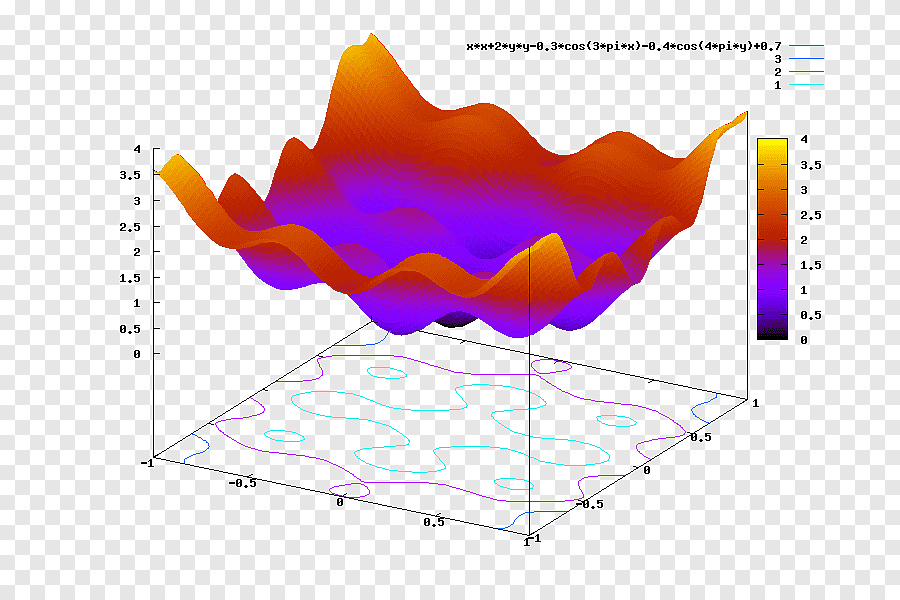
\includegraphics[scale=0.25]{img/page_de_garde.png} \\[1cm]
        \HRule \\[0.4cm]
        { \huge \bfseries LINMA2471 Optimization models and methods II \\[0.4cm] }
    
        \HRule \\[1.5cm]
        \textsc{\LARGE Simon Desmidt}\\[1cm]
        \vfill
        \vspace{2cm}
        {\large Academic year 2024-2025 - Q1}
        \vspace{0.4cm}
         
        
\includegraphics[width=0.15\textwidth]{img/epl.png}
        
        UCLouvain\\
    
    \end{center}
    \end{sffamily}
\end{titlepage}

\setcounter{tocdepth}{1}
\tableofcontents
\chapter{Gradient Method}
An optimization problem is defined as 
\begin{equation}\label{eq:1}
    \min_{x\in \mathbb{R}^n} f(x)
\end{equation}
where \(f:\mathbb{R}^n\rightarrow\mathbb{R}\) is a continuously differentiable function. 
\section{Definitions}
\begin{itemize}
    \item A function \(F:\mathbb{R}^n\rightarrow \mathbb{R}^n\) is L-Lipschitz continuous when \[\lVert F(y)-F(x)\rVert \le L\lVert y-x\rVert\qquad \forall x,y\in \mathbb{R}^n\]where we use the euclidian norm. 
    \item If \(\nabla f\) is L-Lipschitz then, given \(x\in \mathbb{R}^n\), \[f(y)\le f(x)+\langle \nabla f(x), y-x\rangle +\frac{L}{2}\lVert y-x\rVert^2 = m_x(y)\qquad \forall y\in \mathbb{R}^n\]and \(f\) is said to be a L-smooth function.
    \item We say that a differentiable function \(\Psi:\mathbb{R}^n\rightarrow \mathbb{R}\) is L-smooth for some \(L\ge 0\) when, given \(x\in \mathbb{R}^n\), \[\Psi(y) \le \Psi(x) + \langle \nabla \Psi (x),y-x\rangle + \frac{L}{2}\lVert y-x\rVert^2 \qquad \forall y\in \mathbb{R}^n\]
    \item A convex function \(f:\mathbb{R}^n \rightarrow \mathbb{R}\) is convex when, given \(x,y\in \mathbb{R}^n\) and \(\lambda \in [0,1]\), we have \[f(\lambda x+(1-\lambda)y)\le \lambda f(x)+(1-\lambda)f(y)\]
    \item Let \(f:\mathbb{R}^n\rightarrow\mathbb{R}\) be convex. If \(f\) is differentiable, then \[f(y) \ge f(x) + \nabla f(x)^T (x-y) \qquad \forall x,y\in \mathbb{R}^n\]
    \item A differentiable function \(f:\mathbb{R}^n\rightarrow \mathbb{R}\) is \(\mu\)-strongly convex \((\mu>0)\) if, given \(x\in \mathbb{R}^n\), \[f(y) \ge f(x) + \nabla f(x)^T(y-x) + \frac{\mu}{2}\lVert y-x\rVert^2 \qquad \forall y\in \mathbb{R}^n\]
    \item PL inequality for a \(\mu\)-strongly convex function\footnote{\(x^*\) is the minimizer of \(f\)}: \[f(x)-f(x^*)\le \frac{1}{2\mu} \lVert \nabla f(x)\rVert^2 \qquad \forall x\in \mathbb{R}^n\]
\end{itemize}
% \section{Complexity of GM for non convex functions}
% A function \(F:\mathbb{R}^n\rightarrow \mathbb{R}^n\) is L-Lipschitz continuous when \[\lVert F(y)-F(x)\rVert \le L\lVert y-x\rVert\qquad \forall x,y\in \mathbb{R}^n\]where we use the euclidian norm. \\
% In what follows, let us consider the assumption A1 that \(\nabla f\) for \(f\) in equation \ref{eq:1} is L-Lipschitz, i.e. \[\lVert \nabla f(y)-\nabla f(x)\rVert \le L\lVert y-x\rVert\qquad \forall x,y\in \mathbb{R}^n\] \\
% Lemma 1 : If \(\nabla f\) is L-Lipschitz then, given \(x\in \mathbb{R}^n\), \[f(y)\le f(x)+\langle \nabla f(x), y-x\rangle +\frac{L}{2}\lVert y-x\rVert^2 = m_x(y)\qquad \forall y\in \mathbb{R}^n\]and \(f\) is said to be a L-smooth function.\\
% Definition 2 : We say that a differentiable function \(\Psi:\mathbb{R}^n\rightarrow \mathbb{R}\) is L-smooth for some \(L\ge 0\) when, given \(x\in \mathbb{R}^n\), \[\Psi(y) \le \Psi(x) + \langle \nabla \Psi (x),y-x\rangle + \frac{L}{2}\lVert y-x\rVert^2 \qquad \forall y\in \mathbb{R}^n\]
% \begin{itemize}
%     \item [\(\rightarrow\)] N.B. : Any function with L-Lipschitz gradient is L-smooth.
% \end{itemize}
% Using iterations, we can show that the gradient method is, given \(x_0\in \mathbb{R}^n\), 
% \begin{equation}
%     x_{k+1} = x_k-\frac{1}{L}\nabla f(x_k)
% \end{equation}
% Let us suppose that \(f\) is non convex and that (A2) there exists \(f_{low}\in \mathbb{R}\) such that \(f(x)\ge f_{low} \qquad \forall x\in \mathbb{R}^n\).\\
% From lemma 1 and A1, we can now write
% \begin{equation}
%     f(y) \le f(x) + \langle \nabla f(x),y-x\rangle + \frac{L}{2}\lVert y-x\rVert^2 \qquad x,y\in \mathbb{R}^n
% \end{equation}
% In particular, for \(x=x_k\) and \(y=x_{k+1}\), we have
% \begin{equation}
%     f(x_{k+1}) \le f(x_k) - \frac{1}{2L}\lVert \nabla f(x_k)\rVert^2\Longrightarrow f(x_k)-f(x_{k+1}) \ge \frac{1}{2L}\lVert f(x_k)\rVert^2
% \end{equation}
% Defining a given number \(T\ge 1\), we have 
% \begin{equation}
%     f(x_k)-f(x_{k+1}) \ge \frac{1}{2L}\lVert f(x_k)\rVert^2 \qquad \forall k=0,\dots, T-1
% \end{equation}
% Thus, by some algebraic manipulations, we can write 
% \begin{equation}\label{eq:2}
%     \min_{l=0,\dots,T-1} \lVert \nabla f(x_l)\rVert^2 \le \frac{2L}{T}\left(f(x_0)-f_{low}\right) \Longrightarrow \min_{l=0,\dots,T-1} \lVert \nabla f(x_l)\rVert \le \frac{\sqrt{2L\left(f(x_0)-f_{low}\right)}}{\sqrt{T}} = \mathcal{O}\left(\frac{1}{\sqrt{T}}\right) 
% \end{equation}
% This means that, given \(\varepsilon >0\), there exists \(T_0\in \mathbb{N}\) such that \(\min_{l=0,\dots,T-1}\lVert \nabla f(x_l) \rVert \le \varepsilon \qquad \forall T\ge T_0\), i.e. \(\exists l\in \{0,\dots,T-1\}\) such that \(\lVert \nabla f(x_l) \rVert \le \varepsilon\) whenever \(T\ge T_0\). \\
% Now, given \(\varepsilon>0\), we define \(T(\varepsilon) = \min \left\{k\in \mathbb{N}:\lVert \nabla f(x_k)\rVert \le \varepsilon\right\}\). Let us suppose that \(T(\varepsilon)\ge 1\). Then, by equation \ref{eq:2}, 
% \begin{equation}
%     \varepsilon < \min_{l=0,\dots,T(\varepsilon)-1} \lVert\nabla f(x_l)\rVert \le \sqrt{\frac{2L(f(x_0)-f_{low})}{T(\varepsilon)}}
% \end{equation}
% And by algebraic manipulations,
% \begin{equation}
%     T(\varepsilon)\le 2L(f(x_0)-f_{low}) \varepsilon^{-2} = \mathcal{O}(\varepsilon^{-2})
% \end{equation}
% This means that the gradient method applied to a non convex function takes no more than \(\mathcal{O}(\varepsilon^{-2})\) iterations to find an \(\varepsilon\)-approximate stationary point.
\section{Complexity}
The demonstration of the final results here obtained is in the notes, but not explained here. 
\subsection{Hypotheses}
\begin{itemize}
    \item \(f\) is convex and differentiable;
    \item \(\nabla f\) is L-Lipschitz;
    \item we start from a \(x_0\in \mathbb{R}^n\) that is not a minimizer of \(f\);
\end{itemize}
\subsection{Results}
We use the sequence \(\{x_k\}_{k\ge 0}\), given a \(x_0\in \mathbb{R}^n\), such that \[x_{k+1} = x_k - \frac{1}{L}\nabla f(x_k)\]
\begin{center}
    \begin{tabular}{c|c|c}
    Problem class & Goal & Complexity bound \\ \hline\hline
    Non-convex \(f\) & \(\lVert \nabla f(x_k)\rVert \le \varepsilon\) & \(\mathcal{O}(\varepsilon^{-2})\)\\ \hline
    Convex \(f\) & \(f(x_k)-f(x^*)\le \varepsilon\) & \(\mathcal{O}(\varepsilon^{-1})\)\\ \hline
    \(\mu\)-strongly-convex \(f\) & \(f(x_k)-f(x^*)\le \varepsilon\) & \(\mathcal{O}(\log (\varepsilon^{-1}))\)
\end{tabular}
\end{center}
\section{GM with Armijo Line Search}
The Armijo Line Search consists of changing the constant in the GM in order to be more efficient and be able to make bigger steps in some directions where it is possible. 
\begin{equation}
    x_{k+1} = x_k - \alpha \nabla f(x_k)\qquad \alpha >0
\end{equation}
\begin{algorithm}\label{algo:Armijo}
    \caption{Gradient Method with Armijo Line Search}
    \begin{algorithmic}[1]
    \State \textbf{Step 0:} Given $x_0 \in \mathbb{R}^n$ and $\alpha_0 > 0$, set $k \coloneqq 0$.
    \State \textbf{Step 1:} Set $\ell \coloneqq 0$.
    \State \textbf{Step 1.1:} Compute $x_k^+ = x_k - (0.5)^\ell \alpha_k \nabla f(x_k)$.
    \State \textbf{Step 1.2 (Armijo Line Search):} If
    \[
    f(x_k) - f(x_k^+) \geq \frac{(0.5)^\ell \alpha_k}{2} \|\nabla f(x_k)\|^2 \tag{1}
    \]
    set $\ell_k \coloneqq \ell$ and go to Step 2. Otherwise, set $\ell \coloneqq \ell + 1$ and go back to Step 1.1.
    \State \textbf{Step 3:} Define $x_{k+1} = x_k^+$, $\alpha_{k+1} = (0.5)^{\ell_k - 1} \alpha_k$, set $k \coloneqq k + 1$ and go back to Step 1.
    \end{algorithmic}
\end{algorithm}
\section{Problems with convex constraints}
Consider the problem
\begin{equation}\label{eq:convex_problem}
    \min_{x\in \mathbb{R}^n} f(x) \text{ such that } x\in \mathbb{\Omega}
\end{equation}
where \(f\) is L-smooth, and \(\Omega \subseteq \mathbb{R}^n\) is nonempty, closed and convex.
Given an approximation \(x_k\in \Omega\) for a solution of \ref{eq:convex_problem}, a possible generalization of the Gradient Method is to define 
\begin{equation}
    x_{k+1} = P_{\Omega} \left(x_k-\frac{1}{L}\nabla f(x_k)\right)
\end{equation}
where \(P_{\Omega}\) is the projection of \(z\) onto \(\Omega\), and we call this method the Projected Gradient Method.\\
If \(\Omega = [a,b]^n\), then the projection of an element \(z\) onto \(\Omega\) is such that its element \(i\) is given by:
\begin{equation}
    \left[P_\Omega(z)\right]_i = \begin{cases}
        z_i \text{ if } a\le z_i\le b\\
        a \text{ if } z_i<a\\
        b \text{ if }z_i>b\\
    \end{cases} \qquad \forall i=1,\dots,n
\end{equation}
\end{document}